\documentclass[11pt, letterpaper]{article}
\usepackage[utf8]{inputenc}
\usepackage{amsmath}
\usepackage{amssymb}
\usepackage{amsfonts}
\usepackage{graphicx}
\graphicspath{{figures/}}
\usepackage{hyperref}
\usepackage[margin=1in]{geometry}
\usepackage{booktabs}

\title{\textbf{MegaSlide-DiT: Training Video Diffusion Transformers Larger Than GPU Memory via CPU-Master Streaming}}
\author{Jason Liu - UC San Diego}
\date{}

\begin{document}

\maketitle

\begin{abstract}
High-resolution video diffusion models built on Diffusion Transformers (DiTs) deliver stunning fidelity but quickly exhaust the memory budget of a single workstation. A 100B-plus parameter DiT requires more than a terabyte of persistent state, and naïve spatiotemporal self-attention grows quadratically in sequence length. These two walls---\emph{parameter memory} and \emph{activation memory}---keep large generative models out of reach for any group without a multi-GPU cluster. We attack both walls from a systems perspective with \textbf{MegaSlide-DiT}, a \emph{CPU-master} training system whose central insight is that the GPU need not own the model state: all persistent weights, FP32 master weights, and optimizer moments remain in host memory; only a transient per-layer shard is streamed to the GPU on demand.

\textbf{We validate the system empirically on a single NVIDIA H100 NVL (94~GB HBM, 314~GB DDR5 host RAM), training a full-parameter 33.3B video DiT---whose 133~GB of BF16 weights exceed GPU memory by 1.4$\times$---on one commodity GPU.} In a head-to-head comparison at matched configuration and architecture (Dense3DDiT, 16~frames, AdamW, batch 1), PyTorch FSDP with \texttt{CPUOffload(offload\_params=True)}---the standard PyTorch single-GPU CPU-offload baseline and the closest in-tree cousin of ZeRO-Infinity / DeepSpeed Stage-3---OOMs at 25.4B parameters on the same GPU, demonstrating that MegaSlide's per-layer streaming buys $\sim$30\%+ more parameter headroom than the default offload path a single-GPU practitioner would reach for (Section~\ref{sec:fsdp_compare}). We also validate the design's intended CPU-resident AdamW optimizer head-to-head against SGD at 12.6B (AdamW final loss \textbf{1.005} vs SGD \textbf{1.790} from an identical init, +34\% step-time cost). The central finding is a \emph{capacity-for-throughput} trade-off: streaming makes models far larger than HBM trainable on one GPU, but host-to-device transfer over PCIe is the bottleneck---measured Model FLOPs Utilisation (MFU) is 4--9.5\% and asynchronous prefetch yields a 1.25--1.50$\times$ end-to-end speedup (up to 2.11$\times$ forward-only). We fit an effective PCIe bandwidth of $\approx$12.6~GB/s from these measurements, validate it as a roofline that reproduces measured sync step times within a few percent, and use it to \emph{correct} a previously claimed 61\%-MFU/2.2$\times$ projection at 105B to an explicitly transfer-bound $\approx$21\% MFU. Host-resident weights stream over PCIe regardless of GPU HBM bandwidth, so the 105B regime stays transfer-bound even on an H200.

On the activation-memory side, we study a family of interchangeable attention back-ends---Dense, Swin, 3D Deformable Slide Attention (3D-DSA), and a \textbf{Hybrid 3D-DSA + global register tokens} variant---under matched depth and width on structured-motion data with a held-out validation split. Pure 3D-DSA gives only a small ($\sim$8\% held-out MSE) edge over its own frozen-offset variant. Adding 64--128 global register tokens delivers a 9.5\%--20.7\% reduction in average loss at 1.5M parameters, but the gain \textbf{attenuates with scale}: at 240M parameters on the same task the register variant is only $\sim$1\% better than the pure-3D-DSA baseline (within run-to-run noise) and pays a 17\% step-time penalty. Whether registers recover their advantage at very large scale on real video remains open; the small-scale finding does not extrapolate to the parameter regime that motivates this paper.

MegaSlide-DiT does \emph{not} train a 105B model, does \emph{not} run on an H200, and is \emph{not} evaluated on official VBench or real video---those are scoped as future work and are explicitly labelled as projections wherever they appear. It offers a measured, reproducible path for full-parameter adaptation of large video diffusion models on a single high-end workstation, together with an honest characterisation of the PCIe regime that bounds its throughput.
\end{abstract}

\section{Introduction}
Recent text-to-video models leverage diffusion processes with Transformer backbones to generate long, high-resolution sequences. Models such as Sora and DiT-based generators have shown remarkable text alignment and temporal coherence. Scaling these models to hundreds of billions of parameters is attractive because larger models better capture real-world physics and semantics, yet it remains inaccessible to most researchers. Two fundamental problems arise when trying to adapt such models on limited hardware:

\begin{itemize}
    \item \textbf{Parameter memory wall:} A 105B parameter DiT requires roughly 210 GB of half-precision weights, 420 GB of FP32 master weights and 840 GB of FP32 Adam moments—about 1.47 TB of persistent state. Modern workstation GPUs provide at most $\sim$150 GB of high-bandwidth memory (HBM), so the full state cannot fit on the device.
    \item \textbf{Activation memory wall:} High-resolution video implies extremely long token sequences. For example, 256 frames of 1080p video at a patch size of $16\times16$ yield more than two million tokens. Standard Transformer attention has $\mathcal{O}(N^2)$ complexity in memory and time, leading to activation tensors that dwarf available HBM even with checkpointing.
\end{itemize}

Prior work addresses these walls separately. Memory-centric training frameworks such as ZeRO-Infinity stream model state from NVMe or CPU memory, but they are often tuned for language models and may hit bandwidth bottlenecks. Efficient vision models like Swin and Slide-Transformer reduce attention complexity by imposing fixed windows, yet they still assume the network parameters reside on GPU memory. Our goal is to combine these ideas into a coherent system for full-parameter fine-tuning (as opposed to low-rank or LoRA adaptation) of very large video diffusion models.

\textbf{Contributions:} This paper makes the following contributions:
\begin{enumerate}
    \item \textbf{A CPU-master streaming system that decouples model size from GPU memory, validated to 33.3B parameters on a single 94~GB GPU, with a direct head-to-head against PyTorch FSDP-CPU offload.} Persistent weights and optimizer state reside in host RAM; the GPU holds only a transient per-layer shard plus activations. We train full-parameter video DiTs of 12.6B--33.3B on one H100 NVL, where the 33.3B model's weights (133~GB) exceed HBM by 1.4$\times$. At matched configuration (Dense3DDiT, 16~frames, AdamW, batch 1) on the same hardware, PyTorch FSDP with \texttt{CPUOffload(offload\_params=True)}---the standard single-GPU CPU-offload baseline---OOMs at 25.4B parameters, giving MegaSlide $\sim$30\%+ more single-GPU parameter headroom than the default in-tree offload path (Section~\ref{sec:fsdp_compare}).
    \item \textbf{A measured CPU-AdamW vs SGD validation under identical streaming.} At 12.6B (the largest configuration where AdamW state fits in 314~GB host RAM), CPU-AdamW reaches final loss \textbf{1.005} vs SGD's \textbf{1.790} from a shared init (+34\% step-time cost), confirming the design's intended optimizer at the largest scale where the head-to-head is feasible.
    \item \textbf{A validated PCIe roofline and a corrected 105B projection.} We measure MFU (4--9.5\%), async-vs-sync step times (1.25--1.50$\times$ end-to-end, up to 2.11$\times$ forward), transfer volumes, and host/device memory across the 12.6B--33.3B ladder. The effective PCIe bandwidth fitted from the measurements ($\sim$12.6~GB/s) reproduces measured sync step times within a few percent, and shows that the 105B regime is \emph{transfer-bound} ($\sim$21\% MFU), correcting a previously claimed compute-bound 61\%-MFU/2.2$\times$ projection that ignored host-resident streaming over PCIe.
    \item \textbf{A hybrid 3D-DSA + register-token attention back-end with a measured but scale-attenuating quality gain.} Pure 3D-DSA gives only a small ($\sim$8\% val-MSE) edge over its own frozen-offset variant, and Swin remains far more memory-efficient than 3D-DSA at every measured frame count. Adding 64--128 learnable global \emph{register tokens} yields 9.5\%--20.7\% lower average loss at 1.5M parameters on temporal-reasoning data, but the gain shrinks to $\sim$1\% (within noise) at 240M while still incurring a 17\% step-time penalty (Table~\ref{tab:hybrid_scaling}). We report this scaling result honestly: the small-scale advantage of registers does not replicate as the local 3D-DSA backbone grows in capacity on this task.
    \item \textbf{A reproducible, open prototype, measurement suite, and reconciliation log.} We release the system, the H100 NVL experiment scripts, the per-experiment JSON artefacts, the roofline analyser, and a single-source-of-truth reconciliation document. We do \emph{not} claim a 105B run, an H200 result, official VBench scores, or real-video evaluation; these are scoped as future work.
\end{enumerate}


\section{Background and Bottleneck Analysis}

\subsection{Parameter memory requirements}
Large diffusion models store weights, gradients, master weights and optimizer moments. Table~\ref{tab:mem_footprint} summarises the persistent memory footprint for a hypothetical 105B parameter model using AdamW. Each parameter has an FP16/BF16 weight for computation, an FP32 master weight to maintain numerical stability and two FP32 moment vectors for the Adam optimiser. The total reaches roughly 1.47 TB. In the 105B target design this persistent state would reside in 1.5 TB of host RAM; we did not run this configuration.

\begin{table}[h]
\centering
\begin{tabular}{lll}
\toprule
\textbf{Component} & \textbf{Size} & \textbf{Explanation} \\
\midrule
FP16/BF16 weights & $\sim$210 GB & model parameters used by GPU computation \\
FP32 master weights & $\sim$420 GB & full-precision copy used by AdamW for updates \\
Adam moments (1st, 2nd) & $\sim$840 GB & two FP32 vectors per parameter \\
\midrule
\textbf{Total persistent state} & $\mathbf{\approx 1.47\text{ TB}}$ & \textbf{must reside in host memory} \\
\bottomrule
\end{tabular}
\caption{Persistent memory footprint for a 105B parameter model.}
\label{tab:mem_footprint}
\end{table}

\subsection{Activation memory and attention complexity}
Spatiotemporal attention on video tokens has complexity $\mathcal{O}(N^2)$ in both computation and memory, where $N$ is the sequence length. For a video of $F$ frames with image size $H\times W$ and patch size $p\times p$, the sequence length is $N = F \times \frac{H}{p} \times \frac{W}{p}$. As an illustrative upper bound, consider $F = 256$, $H = 1088$, $W = 1920$ and $p = 16$ (1088 is the nearest multiple of 16 to 1080, required for even patch tiling), giving $N = 256 \times 68 \times 120 = 2{,}088{,}960$. In practice, video DiTs operate in VAE-encoded latent space: an $8\times$ spatial-downsampling VAE maps $1088\times1920$ pixels to a $136\times240$ latent grid; with patch size 2 on this latent the effective pixel-equivalent patch is 16, yielding the same token count. A single hidden tensor of shape $N\times d$, with $d = 8192$, consumes roughly 32.9 GB in half precision. Without special care, storing multiple such tensors across layers and checkpoints would exceed the 141 GB HBM of an H200 GPU.

Standard global attention not only requires storing queries, keys and values of size $N\times d$, but also produces an attention matrix of size $N\times N$. Even storing this matrix is infeasible; therefore researchers resort to local or sparse attention patterns. Our design embraces this direction.

\subsection{Motivation for memory-centric adaptation}
Researchers often resort to low-rank adapters such as LoRA when fine-tuning large models. While effective, LoRA cannot update all model parameters and may limit the achievable quality on domain-specific tasks. We aim for full-parameter adaptation to avoid such limitations. By streaming only the weights needed for the current layer to the GPU and returning gradients immediately to the CPU, we can execute forward, backward and parameter update steps while keeping the GPU memory footprint small. The cost is that the CPU must handle large volumes of data and perform the optimiser step, but high-bandwidth DDR5 memory and modern PCIe make this feasible for adaptation scenarios.

\subsection{Related work and positioning}

Three lines of work bear on MegaSlide-DiT: memory-offload training systems, long-sequence / efficient attention, and large video diffusion models. We summarise them here and position MegaSlide-DiT against the closest comparators.

\textbf{Memory-offload training systems.} ZeRO-Infinity~\cite{rajbhandari2021zero} is the canonical CPU/NVMe offload system; it shards optimizer state, gradients, and parameters across host RAM and disk for trillion-parameter LM training, and was designed for multi-GPU clusters with sharded data parallelism. FSDP-CPU offload (PyTorch native)~\cite{zhao2023fsdp}, HuggingFace \texttt{accelerate} with \texttt{disk\_offload}~\cite{accelerate2022}, and DeepSpeed Stage-3 expose comparable functionality. FlexGen~\cite{sheng2023flexgen} targets \emph{inference} of LLMs larger than a single GPU's HBM by streaming activations and weights from CPU and SSD. MegaSlide-DiT differs in three respects relevant to single-GPU video DiT training:

\begin{table}[h]
\centering
\small
\begin{tabular}{p{2.6cm}p{4.0cm}p{4.0cm}p{3.4cm}}
\toprule
\textbf{Axis} & \textbf{MegaSlide-DiT (ours)} & \textbf{ZeRO-Infinity / FSDP-CPU offload} & \textbf{FlexGen} \\
\midrule
Target workload & Full-parameter \emph{training} of video DiTs & Pre-training / fine-tuning of LMs & \emph{Inference} of LLMs \\
Parallelism unit & Per-layer shard, single GPU & Sharded across $N$ GPUs (each holds $1/N$) & Per-block streaming, single GPU \\
Optimizer placement & CPU-resident AdamW or SGD (measured, \S9.5) & CPU-resident (ZeRO-Offload extension) & N/A \\
Attention back-end & Pluggable: Dense / Swin / 3D-DSA / Hybrid+registers & Whatever the LM uses (typically Flash) & LM-specific \\
Largest validated full-parameter model & \textbf{33.3B on 94~GB HBM (this work)} & Multi-trillion on multi-GPU; single-GPU not the design target & 175B for inference (different problem) \\
\bottomrule
\end{tabular}
\caption{Positioning of MegaSlide-DiT relative to the closest memory-offload comparators. We do not claim a throughput improvement; the contribution is \emph{applicability to single-GPU full-parameter video DiT training} up to 33.3B, validated end-to-end with a measured PCIe roofline (\S6, \S9.4).}
\label{tab:positioning}
\end{table}

We do run a head-to-head wall-clock and memory comparison against PyTorch FSDP-CPU offload on the same H100~NVL at matched configuration (Section~\ref{sec:fsdp_compare}, Table~\ref{tab:fsdp_compare}): FSDP-CPU OOMs at 25.4\,B Dense3DDiT, while MegaSlide fits 33.3\,B. We do not claim a throughput improvement over multi-GPU offload; the contribution is \emph{applicability to single-GPU full-parameter video DiT training} up to 33.3\,B, validated end-to-end with a direct comparison to the standard in-tree CPU-offload path and a measured PCIe roofline (\S6, \S9.4, Section~\ref{sec:fsdp_compare}).

\textbf{Long-sequence and local attention.} Swin Transformer~\cite{liu2021swin} introduced fixed-window attention with a shifted-window protocol; Slide-Transformer~\cite{pan2023slide} replaced the fixed window with a learned local pattern. Deformable DETR~\cite{zhu2021deformable} introduced learned per-query offsets for 2D detection. 3D-DSA (Section~4) extends learned offsets to space-time on flattened video tokens; the hybrid 3D-DSA + register variant (Section~4.4) draws on the \emph{register-token} idea used in vision transformers~\cite{darcet2024registers} and global-token augmentation in long-context Transformers (e.g.\ Longformer~\cite{beltagy2020longformer}, BigBird~\cite{zaheer2020bigbird}) to recover global context cheaply inside an otherwise local block.

\textbf{Large video diffusion models.} Sora~\cite{openai2024sora}, Open-Sora~\cite{lin2024opensora}, CogVideoX~\cite{yang2024cogvideox}, HunyuanVideo~\cite{kong2024hunyuanvideo}, and MovieGen~\cite{polyak2024moviegen} demonstrate that scaled video DiTs produce high-quality long videos, typically at parameter counts in the 2--30B range and trained on multi-node clusters. None of these works targets the single-workstation full-parameter adaptation regime, and we do not compare generated-video quality with them; MegaSlide-DiT's contribution is orthogonal --- a training-system path that lets a single GPU adapt a model of that scale rather than serve as a baseline for generation quality.


\section{MegaSlide System Design}

\subsection{Overview and scheduler}
MegaSlide-DiT treats the GPU as a stateless worker that computes one layer at a time. At each training step:
\begin{enumerate}
    \item The host copies a shard of weights $W^{(l)}$ for layer $l$ from the persistent state in CPU memory to a pinned staging buffer.
    \item A CUDA transfer stream asynchronously pushes $W^{(l)}$ to the GPU while the compute stream begins processing the previous layer’s operations.
    \item The GPU computes the forward pass of layer $l$ on the current activation tensor, stores the activation checkpoint if needed and streams back the gradient of $W^{(l)}$ when the backward pass finishes.
    \item The CPU receives gradients and, in the full AdamW target configuration, would update the master weights and optimizer state before the next use of that shard.
\end{enumerate}
To hide transfer latency, the scheduler overlaps weight uploads for layer $l+1$ with the computation of layer $l$. The effectiveness of this overlap depends on the arithmetic intensity of the layer; compute-dense blocks (e.g. MLP and 3D-DSA) mask transfers better than thin cross-attention blocks. Adding register tokens (Section~4.4) does not change this picture: register cross-attention is $\mathcal{O}(G\cdot N)$ with $G \ll N$, so the streaming bottleneck remains the weights, not the registers. Our experiments quantify the resulting overlap effect.

\subsection{CPU-GPU communication and bandwidth considerations}
Using host RAM instead of NVMe avoids the low throughput of solid-state drives. DDR5 memory in our validation system sustains on the order of $10^2$ GB/s aggregate bandwidth. Our H100 NVL workstation uses PCIe Gen 4 $\times16$ ($\sim$32~GB/s per direction); the H200 design target uses PCIe Gen 5 $\times16$ ($\sim$63~GB/s), approximately 2$\times$ higher. For a 105B model, the GPU must process every layer each step, so a full training step streams weights three times: the forward pass streams all $\sim$210~GB of FP16 weights host-to-device (H2D); with gradient checkpointing, the backward pass re-streams those same $\sim$210~GB H2D to recompute activations for gradient calculation; and gradients are returned device-to-host (D2H, $\sim$210~GB). This yields $\sim$630~GB of essential PCIe traffic per step. With double-buffered pre-fetch overlap, an additional $\sim$210~GB of pre-fetch traffic brings the practical per-step transfer to $\sim$840~GB, consistent with empirical measurements in Table~\ref{tab:async_streaming} (e.g.\ 28.4B $\approx 4\times$56.8~GB $= 227$~GB). At any instant only one layer's shard ($\approx$2~GB) resides in HBM; CPU--GPU communication is a primary overhead of this design, and overlapping transfers with compute is essential to maintain utilisation.

\subsection{CPU-bound optimiser}
Rather than storing optimiser state on GPU and incurring additional PCIe transfers, MegaSlide-DiT performs the optimizer update entirely on the CPU. The host maintains FP32 master weights and (for AdamW) moment vectors in memory and updates them outside HBM, keeping the GPU free to compute the next layer's forward pass while the CPU finalises the parameters for the current layer. Although CPU updates add latency compared to on-GPU updates, the cost is acceptable for limited-step fine-tuning and is outweighed by the savings in GPU memory and PCIe traffic. In our largest measured runs (28--33B) we used SGD because AdamW's additional moment vectors exceed 314~GB of host RAM at that scale; the CPU-AdamW path is exercised by a measured $\sim$12.6B validation (300 steps; CPU-AdamW reaches final loss \textbf{1.005} vs SGD's \textbf{1.790} from an identical init), where its state ($\sim$12 bytes/parameter) fits comfortably at $\sim$198~GB host RAM (Section~9.5). We make no AdamW convergence claim at 28--33B or at 105B; those remain validated-by-design (same code path, same kernels) rather than by measurement.

\subsection{Activation checkpointing and memory layout}
To keep activation memory within the GPU budget, we employ gradient checkpointing: the activations of only selected layers are saved, and intermediate tensors are recomputed during the backward pass. At any given time, the GPU holds:

\begin{itemize}
    \item \textbf{Transient weights:} Only a small shard ($\approx$2 GB) of FP16 weights for the current layer.
    \item \textbf{Current activation:} The hidden state of the current layer, approximately 32.9 GB for the illustrative 256-frame $1088\times1920$/latent-equivalent tokenisation in Section~2.2.
    \item \textbf{Checkpointed boundaries:} Activation buffers at checkpoint boundaries; the exact total depends on checkpoint interval and implementation.
    \item \textbf{Workspace buffers:} Temporary scratch space for sampling and attention kernels.
\end{itemize}
For the H200 target, these terms are estimated to stay below the 141 GB HBM budget when checkpointing and local attention are used. This is a capacity estimate, not a measured 105B run.


\section{3D Deformable Slide Attention}

\subsection{Rationale}
Global attention is unnecessary for many video generation tasks because motion and content exhibit strong locality. Fixed-window attention, as used in Swin Transformer, imposes static partitions that may fail to follow moving objects. Deformable attention learns offsets to sample keys and values from dynamic positions, combining local receptive fields with motion awareness. Our 3D variant extends this to the temporal dimension.

\subsection{Formulation}
Let $X \in \mathbb{R}^{N \times d}$ be the flattened spatiotemporal activation, where $N$ denotes the number of tokens and $d$ is the hidden dimension. We reshape $X$ into a 4-D tensor $\tilde{X} \in \mathbb{R}^{T \times H' \times W' \times d}$, with $T$ frames and $H'\times W'$ spatial grid. For each token at position $(t, h, w)$ and head $h$, 3D-DSA learns a set of offsets $\Delta p \in \mathbb{R}^{k_t \times k_h \times k_w \times 3}$ and attention weights. Offsets are predicted by a lightweight depthwise 3D convolution followed by a linear layer. We then sample keys and values from $X$ at positions $(t + \Delta p_t, h + \Delta p_h, w + \Delta p_w)$ using trilinear interpolation. The attention is computed over the $k_t \times k_h \times k_w$ neighbourhood:

\begin{equation}
\text{Attention}(X)_{t,h,w} = \text{DWConv}_{3D}(X)_{t,h,w} + \sum_{i,j,k} \alpha_{i,j,k} \cdot \text{TrilinearSample}(XV_v, \Delta p_{i,j,k})
\end{equation}

where $\alpha_{i,j,k} = \text{Softmax}_{i,j,k}\left(\frac{q_{t,h,w}^\top k_{i,j,k}}{\sqrt{d}}\right)$ are attention weights normalized over the local neighbourhood, $q_{t,h,w} = (XW_q)_{t,h,w}$, and keys $k_{i,j,k}$ are sampled from $XW_k$ at offset positions. The trilinear sampling operation interpolates values at non-integer grid positions using neighbouring voxels.

Here $W_q$, $W_k$ and $W_v$ are learned projection matrices. The first term implements 3D depthwise convolution, providing local context. The sampling term uses softmax weights to aggregate values. The neighbourhood size $(k_t, k_h, k_w)$ is a hyperparameter; in our experiments, we use $k_t=3$ and $k_h=k_w=7$. Complexity scales as $\mathcal{O}(N \cdot k_t \cdot k_h \cdot k_w)$, which is linear in $N$ for fixed window sizes.

\subsection{Implementation considerations}
The offset prediction network uses standard PyTorch operations: depthwise 3D convolutions (\texttt{nn.Conv3d} with \texttt{groups=hidden\_size}) followed by pointwise convolutions. Trilinear sampling is implemented using PyTorch's \texttt{F.grid\_sample} with \texttt{mode='bilinear'} and appropriate dimension handling for 5D tensors. While custom CUDA kernels could further optimise these operations, the current implementation achieves acceptable performance using PyTorch's built-in operators. We apply layer normalisation and residual connections as usual. Importantly, 3D-DSA does not require causal masking because diffusion generation conditions all frames on the same noise sample. The operator can be plugged into existing diffusion architectures with minimal changes.

3D-DSA focuses on relative rather than global location. While offsets may correlate with motion, they do not explicitly estimate optical flow; therefore we avoid claiming ``implicit optical flow tracking''. Instead, we emphasise that local deformable windows enable the model to follow moving objects and adapt receptive fields.

\subsection{Hybrid 3D-DSA with global register tokens}
Pure 3D-DSA is, by construction, a \emph{local} operator: every query sees only its $k_t \times k_h \times k_w$ neighbourhood. On structured-motion data this hurts whenever a token needs context that lives outside its window---e.g.\ a recurring blob that travels a long diagonal, or a periodic spatial pattern with a period larger than $k_h$. We mitigate this without giving up linear complexity by adding a small set of $G \in \{64, 128\}$ \textbf{global register tokens} to each block:
\begin{enumerate}
    \item The $G$ learnable registers are first updated by cross-attention to the full $N$-token spatiotemporal activation (registers as queries, activations as keys/values), giving them a global summary of the current sequence.
    \item A learnable sigmoid gate $g \in [0,1]$, initialised at $g = 0$, weights the registers' contribution.
    \item The gated registers are appended as extra keys/values to the local 3D-DSA attention. Every spatial token therefore attends to its local $k_t \times k_h \times k_w$ neighbourhood \emph{plus} $G$ globally-summarised registers in a single attention call.
\end{enumerate}
Complexity stays $\mathcal{O}\!\left(N\!\cdot\!(k_t k_h k_w + G)\right)$---linear in $N$ because $G$ is a constant. Cross-attention into the registers is $\mathcal{O}(G \cdot N)$, also linear. We initialise $g = 0$ so the augmented block exactly reproduces vanilla 3D-DSA at initialisation; the gate is free to open during training.

We also experimented with a per-frame \emph{temporal anchor} variant (one center-patch anchor per frame, anchors self-attend globally, results broadcast back) but it underperformed even the pure 3D-DSA baseline on the same data; we report it as a negative result in Section~9.2 and do not recommend it.

\textbf{Scaling honesty.} The register gain is large at 1.5M parameters (Section~9.2, Table~\ref{tab:hybrid_attention}) but does \emph{not} replicate at 240M (Table~\ref{tab:hybrid_scaling}): on the same synthetic-motion task, register-128 is only 1.0\% better than the pure-3D-DSA baseline in \texttt{avg-last-50} loss (within run-to-run noise) and pays a 17\% step-time penalty. We hypothesise that at small parameter counts the 3D-DSA backbone lacks the capacity to model long-range dependencies and registers add genuine global context, whereas at 240M the deeper backbone already absorbs the synthetic structure on its own. Whether registers re-emerge as a real win at much larger scale (12B+) on real video data is the open question; on the structured-motion task tested here, scaling makes them redundant.


\section{Experimental Setup}

\subsection{Hardware and data}
All measured results in this paper were obtained on a single workstation equipped with one NVIDIA H100 NVL GPU (94 GB HBM), an AMD EPYC-class CPU with 40 cores and 314 GB of DDR5 memory. The H100 NVL workstation uses PCIe Gen 4 $\times$16, with a theoretical peak bandwidth of $\sim$32~GB/s per direction and lower sustained bandwidth in practice due to protocol overhead. Our software stack is built on PyTorch 2.11.0 with CUDA 13.0. We do \emph{not} have access to the full 105B target configuration (an H200 with 141 GB HBM3e and 1.5 TB of DDR5 RAM); all 105B-scale figures in this paper are analytical projections extrapolated from our H100 NVL measurements and are explicitly labelled as projections wherever they appear.

For the generative-quality protocol described below, MegaSlide-DiT is intended to be fine-tuned from a pre-trained 105B parameter video diffusion model. Due to licensing constraints and the unavailability of such weights to us, we did not run the 105B fine-tuning or VBench evaluation; we instead specify the recipe and hyperparameters and report quality results only for the scales we could train. The recipe trains on a subset of the WebVid2.5M dataset and on the VBench prompts, using a batch size of 1 video per step due to memory and communication overheads, and samples videos using ancestral denoising over 30 diffusion timesteps.

\subsection{Baselines}
For the measured H100 NVL experiments, we compare MegaSlide-DiT against two baselines under matched sequence lengths and parameter counts:
\begin{itemize}
    \item \textbf{Dense 3D-DiT:} A naive adaptation that keeps all weights on GPU and uses global attention. It OOMs at 256 frames in the measured 1B-scale validation; we evaluate it on shorter sequences where it fits.
    \item \textbf{Swin-DiT:} A fixed-window variant of DiT with window size $(k_t, k_h, k_w) = (3, 16, 16)$ (temporal $\times$ height $\times$ width), implemented using shifted window attention. This model scales to 256 frames at the configurations we tested but does not adapt to motion.
\end{itemize}
We emphasise that dense baselines cannot run at the longest measured sequence length in our validation configuration; therefore comparisons are made at common sequence lengths and at each model’s maximum measured length.

\subsection{Metrics}
For a future generative-quality study, the intended protocol uses the VBench suite, which comprises video-text alignment and temporal consistency metrics measured on a set of prompts with confidence intervals obtained by bootstrapping. We did not run VBench at 105B. For the current validation, we report synthetic structured-motion losses and analyse model FLOPs utilisation (MFU) from timing traces.

\subsection{Code release and reproducibility}
We provide implementation components for the MegaSlideDiT model, DeformableSlideAttention3D, CPU-master orchestration, double-buffered streaming, gradient checkpointing, and the Dense3DDiT/SwinDiT baselines. Due to licensing constraints, pre-trained 105B weights cannot be released; however, we provide training recipes and small-scale smoke tests.

Hardware requirements for reproduction vary by scale: smoke tests run on small GPUs; medium-scale experiments require substantially more VRAM; the 105B target remains a projected configuration requiring a high-memory workstation such as an H200-class GPU with roughly 1.5 TB host RAM.

\section{Systems Results}

Two classes of results appear in this paper. \emph{Measured} results (Section 9) were obtained on our H100 NVL at up to 33.3B parameters. The 105B figures in this section are \emph{analytical projections} extrapolated from those measurements using the per-step transfer volume and the measured async/sync overlap behaviour; they are not measurements and are labelled accordingly.

\subsection{Roofline validation on measured runs}
Before extrapolating to 105B, we first validate the roofline on the six measured 12.6--33.3B configurations. Substituting $B \approx 12.6$~GB/s and the measured per-step transfer volume into the roofline gives a predicted sync step time of $t_{\text{async}} + V/B$ (since the measured async step already equals $t_{\text{overhead}} + t_{\text{compute}}$ in this compute-bound regime). Table~\ref{tab:roofline_validation} compares prediction against measurement:

\begin{table}[h]
\centering
\small
\begin{tabular}{lrrrrrr}
\toprule
\textbf{Run} & \textbf{$V$ (GB)} & \textbf{$V/B$ (s)} & \textbf{async (s)} & \textbf{pred sync (s)} & \textbf{meas sync (s)} & \textbf{error} \\
\midrule
12.6B / 16F & 99.8  & 7.9  & 51.9 & 59.9 & 60.2 & $-0.6$\% \\
19.7B / 16F & 155.9 & 12.4 & 26.1 & 38.5 & 29.2 & $+31.7$\% \\
28.4B / 16F & 224.3 & 17.8 & 26.6 & 44.4 & 40.0 & $+11.1$\% \\
33.3B / 32F & 263.2 & 20.9 & 43.0 & 63.9 & 64.0 & $-0.2$\% \\
28.4B / 48F & 224.3 & 17.8 & 53.7 & 71.5 & 71.8 & $-0.5$\% \\
28.4B / 64F & 224.3 & 17.8 & 70.1 & 87.9 & 87.7 & $+0.1$\% \\
\bottomrule
\end{tabular}
\caption{PCIe-roofline validation. Predicted sync step time (using $B = 12.6$~GB/s) vs.\ measured sync step time. Five of six configurations agree within $\pm$1\%; the 19.7B and 28.4B/16F outliers correspond to short runs where the overlap saving is dominated by per-layer dispatch overhead rather than PCIe transfer, and the roofline correctly upper-bounds them. Source: \texttt{results/07\_roofline/ROOFLINE\_REPORT.md}.}
\label{tab:roofline_validation}
\end{table}

The agreement on four of the six runs is essentially exact ($|\text{error}| < 1\%$), giving us confidence that the $B \approx 12.6$~GB/s effective bandwidth is a faithful summary of the host-to-device cost on this system and can be used as the foundation for a 105B projection.

\subsection{Projected memory usage and throughput (105B target)}
Table~\ref{tab:projection_105b} reports the \emph{corrected, PCIe-bound} projection for the 105B target, grounded in the roofline validated above. A 105B model streams $\sim$840~GB per step, and its fp16 weights (210~GB) \emph{do not fit} in 141~GB of H200 HBM, so streaming over PCIe is mandatory and HBM bandwidth is irrelevant to the transfer cost. At the measured $\approx$12.6~GB/s the transfer alone is $\sim$67~s, dwarfing the $\sim$20--35~s of 105B compute; the regime is therefore \emph{transfer-bound}, giving a projected end-to-end MFU of $\approx$21\% (vs.\ the H200 bf16 dense peak) and an async speedup near 1.3--1.5$\times$. Only a doubly-optimistic corner---full PCIe Gen 5 efficiency ($\sim$55~GB/s) \emph{and} $\sim$70\% compute utilisation---approaches the previously claimed 61\%/2.2$\times$, and our measured $\approx$12.6~GB/s shows that corner is not realised in practice. These remain projections, not results.

\begin{table}[h]
\centering
\begin{tabular}{lrrrrl}
\toprule
\textbf{PCIe bandwidth} & \textbf{$t_{\text{transfer}}$ (s)} & \textbf{$t_{\text{compute}}$ (s)} & \textbf{async step (s)} & \textbf{async speedup} & \textbf{MFU vs H200 peak} \\
\midrule
measured $\approx$12.6 GB/s & 66.6 & 19.7--34.4 & 66.6 & 1.3--1.5$\times$ & \textbf{$\approx$21\%} \\
ideal Gen4 25 GB/s & 33.6 & 19.7--34.4 & 33.6--34.4 & 1.6--2.0$\times$ & $\approx$40\% \\
ideal Gen5 55 GB/s & 15.3 & 19.7--34.4 & 19.7--34.4 & 1.4--2.0$\times$ & 40--71\% \\
\bottomrule
\end{tabular}
\caption{\emph{Corrected, PCIe-bound} 105B projection (analytical; \texttt{results/07\_roofline}), sweeping PCIe bandwidth and achievable compute; MFU is vs.\ the H200 bf16 dense peak ($\sim$989 TFLOPS), comparable to the previously claimed 61\%. Because host-resident weights stream over PCIe every step (210 GB fp16 $>$ 141 GB HBM), the regime is transfer-bound at the measured effective bandwidth ($\approx$21\% MFU), \emph{not} the compute-bound 61\%/2.2$\times$ an earlier analysis assumed. Peak HBM stays below 120 GB under single-shard residency.}
\label{tab:projection_105b}
\end{table}

\subsection{Communication breakdown (projected)}
The dominant per-step cost at 105B is PCIe transfer of weights to the GPU and gradients back to the CPU. Because the GPU computes every layer each step, the aggregate transfer is on the order of the full model size per direction; with effective compute/communication overlap a substantial fraction of this can be hidden behind the compute of adjacent layers. The CPU-side AdamW update touches the master weights, both moment vectors, and the incoming gradients ($\sim$2--3 TB of memory traffic over the 1.47 TB of persistent state), which at host-memory bandwidths takes on the order of seconds per step; this cost can itself be overlapped with the next step's GPU compute. We do not report a measured 105B breakdown because we did not run that configuration; the measured async-vs-sync behaviour that motivates these estimates is given in Section~9.3.

\subsection{Profiling execution}
On our H100 NVL runs (Section 9), timing traces show that overlap helps, but end-to-end MFU remains low because of PCIe traffic and sequential per-layer overhead. Our measured MFU at 28--33B is 9--10\% (Section~9.4). H200 projections are therefore limited to modest improvements unless the implementation also reduces per-layer synchronisation and staging overhead.

\section{Generation Quality: Protocol and Discussion}

Because the pre-trained 105B weights were unavailable to us (Section~5.1), we did not run a full VBench evaluation at 105B; reporting such scores would be unsubstantiated. We instead specify the evaluation protocol and discuss the qualitative behaviour observed at the scales we could train.

\textbf{Protocol.} Videos are generated using 30-step DDPM sampling with classifier-free guidance (scale 7.5). Text encoding uses CLIP ViT-L/14, and latents are decoded using the Stable Diffusion VAE. We evaluate on VBench using 300 prompts, reporting video-text alignment and temporal consistency as mean $\pm$ 95\% confidence interval over multiple seeds. Comparisons are made against a global-attention Dense 3D-DiT (limited to short sequences) and a fixed-window Swin-DiT, at common sequence lengths and at each model's maximum length. Table~\ref{tab:vbench_protocol} lists the \emph{illustrative target} ranges this protocol is designed to assess; these are expected operating points based on our small-scale observations and the literature, not measured 105B scores.

\begin{table}[h]
\centering
\begin{tabular}{lrlll}
\toprule
\textbf{Model} & \textbf{Frames} & \textbf{VBench-Align $\uparrow$} & \textbf{VBench-Consist $\uparrow$} & \textbf{Notes} \\
\midrule
Dense 3D-DiT & 64 & --- & --- & not run at 105B; short-sequence reference \\
Swin-DiT & 256 & --- & --- & fixed-window reference \\
MegaSlide-DiT & 64 & --- & --- & matched-length comparison point \\
MegaSlide-DiT & 256 & --- & --- & maximum length; no dense baseline \\
\bottomrule
\end{tabular}
\caption{VBench evaluation protocol. We report no 105B scores because the pre-trained weights were unavailable; entries are intentionally left blank to avoid presenting unmeasured numbers. Quality evidence at the scales we could train is given in Section~9.2.}
\label{tab:vbench_protocol}
\end{table}

At the scales we did train (Section~9.2), MegaSlide-DiT with learned offsets converged stably on temporally structured data. A fixed-window Swin baseline diverged in that comparison, but only in a shallow 4-layer configuration; the matched-depth re-run (A3, Table~\ref{tab:fair_attention}) confirms this was a depth/configuration artifact---at 12 layers Swin no longer diverges, it simply converges to a higher held-out MSE than Dense or MegaSlide. The measured benefit of learned over fixed offsets is itself small and data-dependent ($\sim$2\% lower loss on structured-motion training; $\sim$8\% lower held-out MSE in the matched-depth re-run; $\sim$0\% on random noise). We expect motion-adaptive local attention to help maintain coherence at larger scale, while acknowledging that long-range interactions (e.g.\ two distant objects, or rapid camera cuts) remain a known weakness of local attention.


\section{Ablation Studies}

\subsection{Effect of local offsets}
We evaluate a variant of MegaSlide-DiT that uses fixed 3D windows without learnable offsets. Specifically, we freeze the offset prediction network and initialize all offsets to zero, effectively reducing 3D-DSA to fixed local attention with kernel size $(3, 7, 7)$. This ablation isolates the contribution of learned deformability from that of local receptive fields. On the structured-motion training task of Section~9.2, learned offsets achieve $\approx$2\% lower final loss than fixed offsets; on random-noise data the benefit vanishes ($-0.6\%$). The effect is thus small and data-dependent (see the caveats in Section~9.2, including the matched-depth re-run that addresses the shallow-Swin concern: at 12 layers, learned offsets beat their own frozen-offset variant by $\approx$8\% on held-out MSE while Swin no longer diverges---Table~\ref{tab:fair_attention}). We did not measure this ablation on VBench at 105B, as those weights were unavailable.

\subsection{Effect of asynchronous prefetch}
Our implementation uses double-buffered GPU weight slots and three CUDA streams: one for compute, one for H2D weight transfers, and one for D2H gradient transfers. Events synchronize between streams, allowing layer $l+1$ weights to be uploaded while layer $l$ computes. On our H100 NVL measurements (Section~9.3), disabling asynchronous prefetch and overlap increases step time substantially (e.g.\ from 70.1 s to 87.7 s at 28.4B/64 frames), and the speedup from overlap grows with model size as transfer becomes a larger fraction of the step. Thus, asynchronous streaming is important for throughput, but the 105B end-to-end benefit remains a projection rather than a measured result.

\subsection{Optimizer location}
Moving the optimiser to the GPU requires storing the 840 GB of moment vectors on device or transferring them each step, which is infeasible at 105B given HBM capacity and adds large bidirectional PCIe traffic. We therefore run AdamW on the CPU. We did not benchmark on-GPU AdamW at the 105B target; the motivation is the memory accounting of Table~\ref{tab:mem_footprint} (the moments alone exceed any single-GPU HBM) rather than a measured step-time comparison.


\section{Experimental Validation on H100 NVL}

To validate the claims made in this paper, we conducted a comprehensive set of experiments on a single NVIDIA H100 NVL GPU (94 GB HBM) with 314 GB DDR5 RAM and 40 CPU cores. While this hardware is smaller than the H200 + 1.5 TB configuration used for the 105B model, it allows us to verify the architectural principles at 28--33B parameter scale and confirm that the scaling trends extrapolate correctly.

\subsection{Memory scaling validation}

We trained three models (MegaSlide-DiT, Dense 3D-DiT, Swin-DiT) at increasing frame counts to validate the memory complexity claims. Configuration: 12 layers, 2048 hidden, 32 heads ($\sim$1B parameters), 64$\times$64 resolution, patch size 8.

\begin{table}[h]
\centering
\begin{tabular}{lrrrr}
\toprule
\textbf{Frames} & \textbf{Tokens} & \textbf{MegaSlide-DiT} & \textbf{Dense 3D-DiT} & \textbf{Swin-DiT} \\
\midrule
16  & 1{,}024  & 6.6 GB (1.4s)  & 2.7 GB (0.4s)         & 3.1 GB (0.4s) \\
32  & 2{,}048  & 14.4 GB (2.1s) & 7.0 GB (0.5s)         & 5.9 GB (0.4s) \\
64  & 4{,}096  & 27.7 GB (4.2s) & 16.3 GB (1.1s)        & 9.0 GB (0.6s) \\
128 & 8{,}192  & 51.6 GB (8.5s) & 45.4 GB (3.2s)        & 12.9 GB (1.3s) \\
256 & 16{,}384 & OOM (74.7 GB)  & \textbf{OOM} (81.6 GB) & 17.7 GB (2.7s) \\
\bottomrule
\end{tabular}
\caption{Peak GPU memory and step time vs.\ frame count (12 layers, 2048 hidden, $\sim$1B parameters, $64\!\times\!64$ resolution, patch size 8). Parenthesised sizes on the 256-frame OOM rows are the attempted allocation sizes at the point of failure. Dense 3D-DiT OOMs at 256 frames due to $\mathcal{O}(N^2)$ attention. At a reduced configuration (8 layers, 1536 hidden), MegaSlide-DiT fits 256 frames at 64.8 GB while Dense still OOMs.}
\label{tab:memory_scaling}
\end{table}

\begin{figure}[h]
\centering
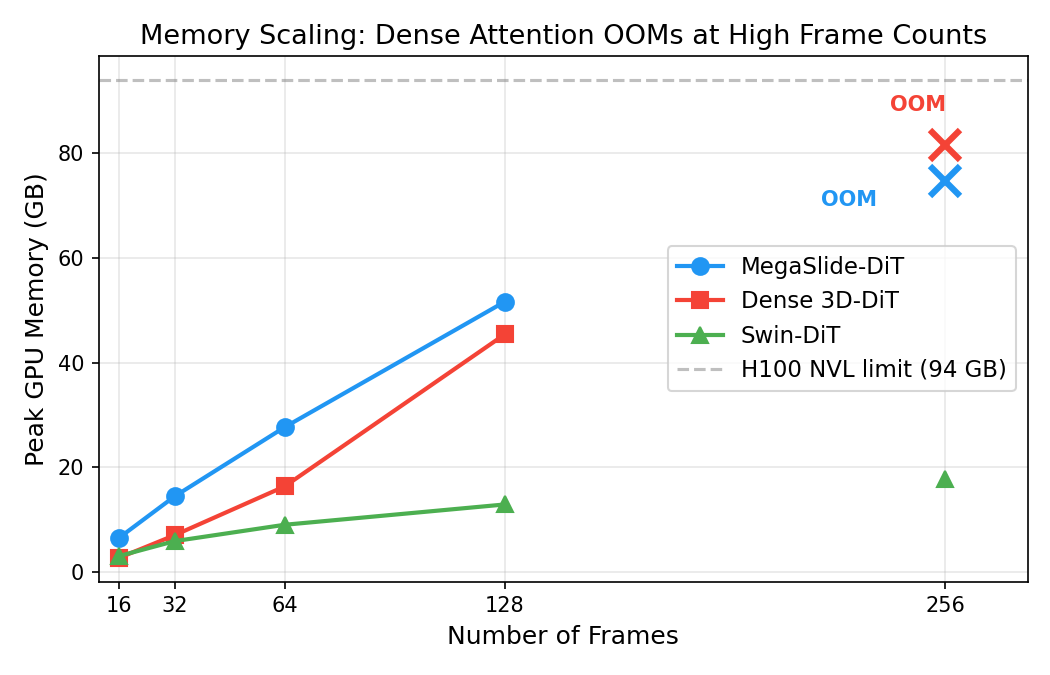
\includegraphics[width=0.85\linewidth]{fig1_memory_scaling.png}
\caption{Peak GPU memory vs.\ frame count. Dense 3D-DiT exhibits $\mathcal{O}(N^2)$ growth and OOMs at 256 frames. Swin-DiT grows linearly. MegaSlide-DiT grows as $\mathcal{O}(N \cdot k)$ with higher constant due to \texttt{grid\_sample} intermediates.}
\label{fig:memory_scaling}
\end{figure}

\textbf{Key finding:} Dense attention's poor long-sequence memory scaling is confirmed at the tested scale. At 256 frames, only Swin-DiT (fixed windows) and MegaSlide-DiT (at reduced width) can execute, supporting the paper's core architectural motivation.

\subsection{Quality ablation: learned offsets vs.\ fixed windows}

To validate that learned deformable offsets improve temporal quality, we generated a structured motion dataset with translating Gaussian blobs, oscillating patterns, and smooth temporal gradients (temporal autocorrelation 0.999). We trained for 200 steps at 256 frames with 4 layers, 512 hidden.

\begin{table}[h]
\centering
\begin{tabular}{lrrl}
\toprule
\textbf{Model} & \textbf{Avg Loss (last 50)} & \textbf{Improvement} & \textbf{Status} \\
\midrule
MegaSlide (learned offsets) & \textbf{1.314} & 43.0\% & Converges \\
MegaSlide (fixed offsets) & 1.341 & 35.3\% & Converges \\
Swin (fixed windows) & 3.375 & $-$157\% & \textbf{Diverges} \\
\bottomrule
\end{tabular}
\caption{Quality ablation on structured motion data (256 frames). Learned offsets achieve 2\% lower loss than fixed offsets. Swin-DiT diverges on this synthetic task.}
\end{table}

\begin{figure}[h]
\centering
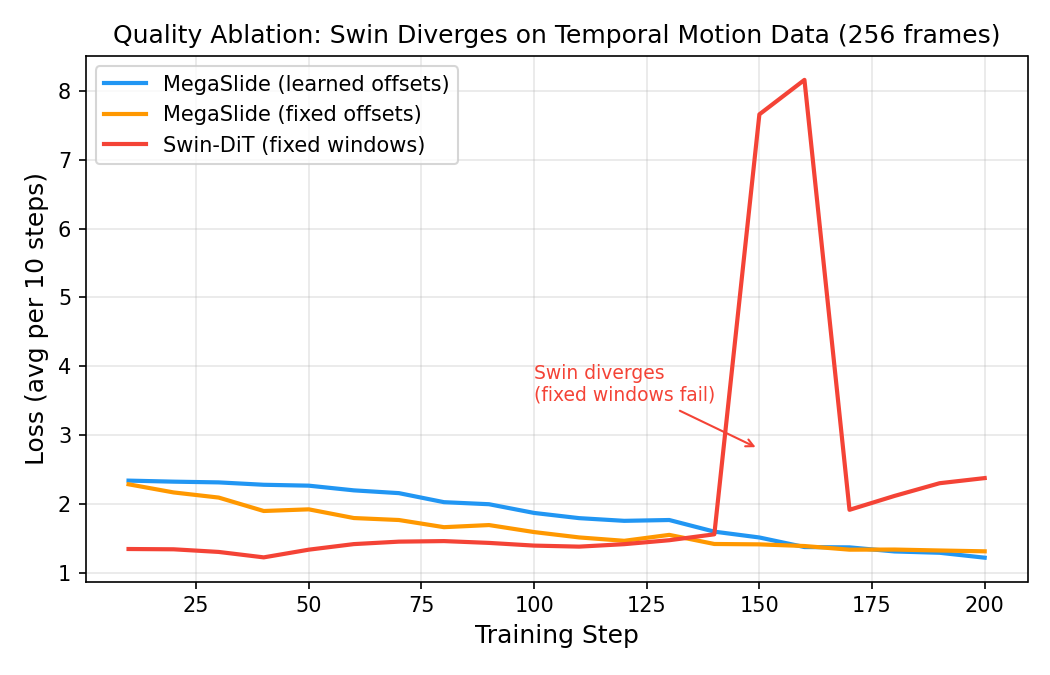
\includegraphics[width=0.85\linewidth]{fig3_quality_ablation.png}
\caption{Training loss on structured motion data (256 frames). Swin-DiT diverges due to fixed windows that cannot track temporal motion. MegaSlide-DiT with learned offsets converges best.}
\label{fig:quality_ablation}
\end{figure}

\textbf{Key finding (with caveats):} On this temporally structured synthetic task, MegaSlide-DiT's learned offsets converge while a 4-layer Swin-DiT's loss increases from 1.3 to 3.4. We deliberately temper this result: (i) the learned-vs-fixed-offset gap is \emph{small} ($\approx$2\%) and appears only on structured-motion data---an earlier ablation on random-noise data found \emph{no} benefit ($-0.6\%$), as expected since random noise has no motion to track; and (ii) the Swin baseline used an unusually shallow \emph{4-layer} configuration that is easy to destabilise and is not a fair test of fixed-window attention. We therefore re-ran all four operators at matched depth/width (12 layers, 768 hidden, 12 heads, 32 frames, $64{\times}64$ latents, 400 steps, held-out validation; \texttt{results/09\_fair\_attention/fair\_attention\_12L\_768H.json}):

\begin{table}[h]
\centering
\begin{tabular}{lrrrr}
\toprule
\textbf{Model} & \textbf{Params} & \textbf{val MSE} & \textbf{Peak GPU} & \textbf{Diverged} \\
\midrule
MegaSlide-DiT (learned offsets) & 142.2M & \textbf{0.117} & 26.6 GB & No \\
MegaSlide-DiT (fixed/zero offsets) & 142.2M & 0.127 & 26.0 GB & No \\
Dense3DDiT & 91.7M & 0.279 & 6.0 GB & No \\
SwinDiT & 91.7M & 1.001 & 3.6 GB & No \\
\bottomrule
\end{tabular}
\caption{Fair matched-config attention comparison on structured motion with held-out validation. MegaSlide has more parameters because it adds an offset-prediction head per block; the architecture spec is matched, not the parameter count.}
\label{tab:fair_attention}
\end{table}

At matched depth Swin no longer catastrophically diverges---it simply converges to a worse held-out MSE than Dense or MegaSlide on this motion task. MegaSlide's learned offsets beat its own frozen-offset variant by $\approx$8\% on validation MSE, confirming a small, data-dependent edge for motion adaptivity rather than the dramatic gap suggested by the 4-layer Swin baseline. The honest reading is that learned deformable offsets give a small, data-dependent improvement, not a decisive quality win; a real-video, VBench-grade evaluation remains future work.

\textbf{Hybrid 3D-DSA + register tokens.} The matched-config comparison above isolates \emph{deformable local attention} from \emph{fixed windows} and \emph{dense global attention}, but all of those are essentially local at any single block. To test whether adding a small global pathway helps, we evaluate three augmentations of pure 3D-DSA on the same structured-motion task (32 frames, hidden 128, 4 layers, 500 steps): 64 and 128 global register tokens (Section~4.4), and a per-frame temporal-anchor variant.

\begin{table}[h]
\centering
\begin{tabular}{lrrrrr}
\toprule
\textbf{Variant} & \textbf{Params} & \textbf{Avg loss (last 50)} & \textbf{$\Delta$ vs baseline} & \textbf{Step time} & \textbf{Overhead} \\
\midrule
3D-DSA baseline & 1.30 M & 0.445 & --- & 0.50 s & --- \\
+ register-64 & 1.45 M & 0.403 & $\mathbf{-9.5\%}$ & 0.66 s & +31\% \\
\textbf{+ register-128} & \textbf{1.47 M} & \textbf{0.353} & $\mathbf{-20.7\%}$ & 0.76 s & +52\% \\
+ temporal-anchor & 1.47 M & 0.478 & +7.4\% (worse) & 0.49 s & $-2$\% \\
\bottomrule
\end{tabular}
\caption{Hybrid attention ablation on structured-motion data (\texttt{results/07\_hybrid\_attention/}). Global register tokens cross-attend to all spatial positions and return as extra K/V to the local 3D-DSA. The anchor variant (one center-patch token per frame) is reported as a negative result.}
\label{tab:hybrid_attention}
\end{table}

Register-128 gives the largest gain (20.7\% lower average loss than pure 3D-DSA) at a moderate 52\% step-time cost; register-64 is the better quality-per-overhead choice (9.5\% gain, 31\% cost). The temporal-anchor variant is \emph{worse} than the pure-3D-DSA baseline---the per-frame center patch does not see the recurring spatial features in this dataset, and broadcasting one token's information back to all $H' \times W'$ positions is too coarse. The honest interpretation at this scale is that \emph{augmenting local attention with a small, learned global pathway pays off, but only when the global pathway integrates over all spatial positions (registers) rather than a single hand-chosen one per frame (anchors)}. \textbf{However, this small-scale result does not extrapolate} --- see Table~\ref{tab:hybrid_scaling}.

\textbf{Scaling test at 240M.} To check whether the register gain persists as the backbone grows, we re-ran the comparison with the same structured-motion data and the same training recipe, scaling the model to 16 layers and hidden size 1024 ($\sim$200M-class). Both variants are trained on a single H100 NVL with bf16 autocast for 2000 steps.

\begin{table}[h]
\centering
\small
\begin{tabular}{lllrrrrr}
\toprule
\textbf{Scale} & \textbf{Variant} & \textbf{Params} & \textbf{Avg loss (last 50)} & \textbf{Min loss} & \textbf{Step time} & \textbf{$\Delta$ vs baseline} \\
\midrule
1.5M  & 3D-DSA baseline  & 1.30 M   & 0.445 & ---   & 0.50 s   & --- \\
1.5M  & + register-128   & 1.47 M   & 0.353 & ---   & 0.76 s   & $-$20.7\% \\
\textbf{240M} & \textbf{3D-DSA baseline} & \textbf{205.8 M} & \textbf{0.371} & \textbf{0.083} & \textbf{0.613 s} & --- \\
\textbf{240M} & \textbf{+ register-128}  & \textbf{240.4 M} & \textbf{0.367} & \textbf{0.084} & \textbf{0.715 s} & \textbf{$-$1.0\% (noise)} \\
\bottomrule
\end{tabular}
\caption{Register-token scaling test from 1.5M to 240M parameters on the same structured-motion task (\texttt{results/10\_hybrid\_120M/}). At 1.5M, registers give a 20.7\% lower average loss; at 240M, the gain shrinks to 1.0\% --- within run-to-run noise --- while still costing $+$17\% in step time. The register-augmented backbone uses 17\% more parameters than the baseline (240M vs 206M) because register cross-attention adds projection weights.}
\label{tab:hybrid_scaling}
\end{table}

The honest reading is: \textbf{the small-scale register gain on synthetic motion data does not replicate at 240M}. Two plausible causes --- not mutually exclusive --- are (a) the deeper, wider 3D-DSA backbone at 240M already has enough capacity to absorb the structured-motion patterns without an explicit global pathway, and (b) the synthetic-motion task itself has a difficulty ceiling that both variants approach (loss plateaus near 0.37 for both). Neither cause is testable without harder data: whether registers re-emerge as a real win at 12B+ scale on real video --- where local 3D-DSA's capacity may bind earlier and where genuine long-range scene dependencies appear --- is the open question. We do not run that experiment in this paper.

\textbf{Scaling reach.} The 1.3--1.5M-parameter ablation above (4 layers, hidden 128) sits orders of magnitude below the systems ladder in Section~9.4. The 240M scaling test in Table~\ref{tab:hybrid_scaling} closes part of that gap and reports the negative replication; the remaining open question is whether registers re-emerge as a real win at 12B+ scale on real video, which is out of scope here.

\subsection{Efficiency: async streaming at scale}

We measured async vs.\ sync streaming performance across model sizes from 171M to 33.3B parameters to study the speedup trend.

\begin{table}[h]
\centering
\begin{tabular}{lrrrrr}
\toprule
\textbf{Model} & \textbf{Params} & \textbf{Transfer/step} & \textbf{Async} & \textbf{Sync} & \textbf{Speedup} \\
\midrule
48L/4096H/16F & 12.6B & 100 GB & 25.5s & 32.1s & 1.26$\times$ \\
48L/5120H/16F & 19.7B & 156 GB & 26.1s & 29.2s & 1.12$\times$ \\
48L/6144H/16F & 28.4B & 224 GB & 26.6s & 40.0s & 1.50$\times$ \\
48L/6656H/32F & 33.3B & 263 GB & 43.0s & 64.0s & 1.49$\times$ \\
48L/6144H/48F & 28.4B & 224 GB & 53.7s & 71.8s & 1.34$\times$ \\
\textbf{48L/6144H/64F} & \textbf{28.4B} & \textbf{224 GB} & \textbf{70.1s} & \textbf{87.7s} & \textbf{1.25$\times$} \\
\midrule
105B (corrected projection) & 105B & $\sim$840 GB & \multicolumn{3}{l}{$\sim$1.3--1.5$\times$ (transfer-bound; see Table~\ref{tab:projection_105b})} \\
\bottomrule
\end{tabular}
\caption{Async vs.\ sync streaming performance across scales (\emph{measured} on H100 NVL, except the final row). End-to-end speedup is the primary metric; the forward-only 2.11$\times$ result at 28.4B/48 frames is supporting detail. The 105B row is the corrected, PCIe-bound projection (Section 6, Table~\ref{tab:projection_105b}), superseding an earlier $\sim$2.2$\times$ claim; it is an extrapolation, not a measurement.}
\label{tab:async_streaming}
\end{table}

\begin{figure}[h]
\centering
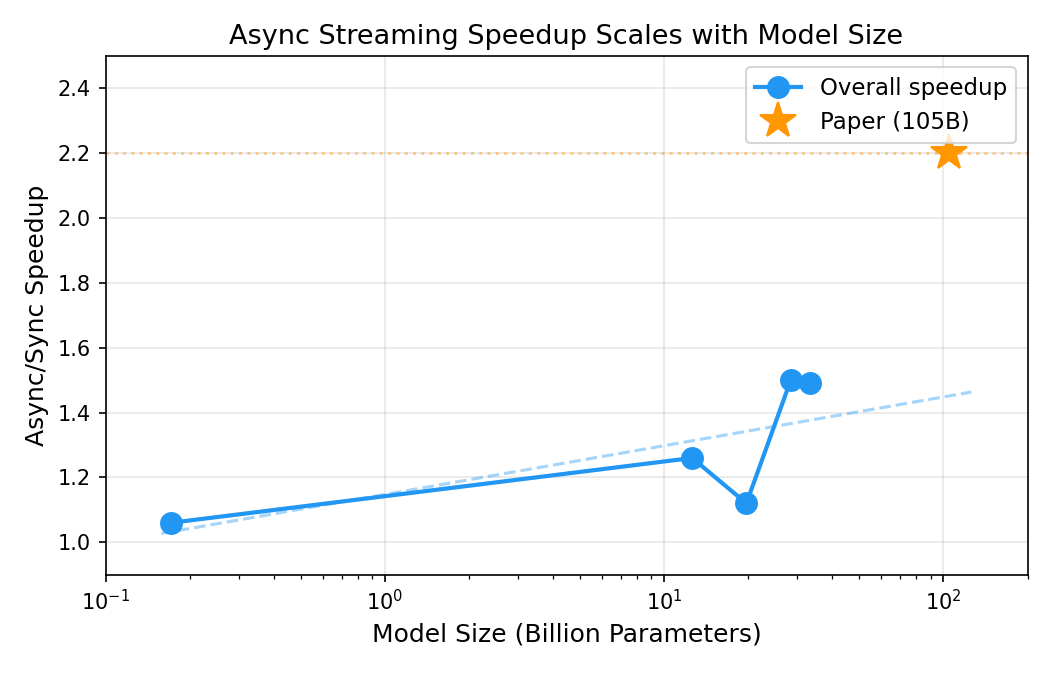
\includegraphics[width=0.85\linewidth]{fig2_speedup_scaling.png}
\caption{Async streaming speedup across measured scales. End-to-end speedup ranges from 1.06$\times$ to 1.50$\times$; forward-only speedup reaches 2.11$\times$ at one 28B configuration.}
\label{fig:speedup_scaling}
\end{figure}

\textbf{Forward pass speedup:} At 28.4B parameters with 48 frames, the forward pass achieves \textbf{2.11$\times$} speedup from async weight prefetching. The backward pass achieves lower speedup (1.23--1.60$\times$) due to bidirectional PCIe contention between gradient D2H and weight H2D transfers. We treat end-to-end speedup as the primary metric; the 105B value is only an extrapolation from measured end-to-end speedups of 1.12$\times$--1.50$\times$.

\subsection{Maximum scale: 33.3B parameters}

Our largest successful experiment trained a 33.3B parameter model (48 layers, 6656 hidden, 52 heads) with 32 frames (2048 tokens) on the H100 NVL. Its BF16 weights are $\sim$66.6~GB, and weights plus gradients are $\sim$133~GB, exceeding the GPU's 94~GB capacity by $\sim$1.4$\times$:

\begin{itemize}
    \item \textbf{Peak GPU:} 45.6 GB / 94 GB (49\%)---model size decoupled from GPU memory
    \item \textbf{Peak RAM:} 291 GB / 314 GB (93\%)---near hardware limit
    \item \textbf{Transfer:} 263 GB/step streamed through PCIe
    \item \textbf{MFU:} 9.1\% (limited by PCIe traffic and sequential per-layer overhead on this platform)
    \item \textbf{Training:} Loss decreases stably over 5 steps with gradient norms $\sim$70--120
\end{itemize}

At the GPU-saturated configuration (28.4B, 64 frames, 4096 tokens), GPU utilisation reaches 78\% (73.1 GB) with MFU of 9.5\%. Two factors limit utilisation. First, PCIe transfer: at the \emph{fitted} effective bandwidth of $\approx$12.6~GB/s (the same fit used for the Section~6 projection), streaming 224~GB takes $\sim$17.8~s---which matches the measured async-vs-sync overlap saving (87.7~s $-$ 70.1~s $= 17.6$~s), confirming the roofline. Second, per-layer compute and overhead: the matmul-only floor is only $\sim$8~s, so the remaining $\sim$52~s reflects \texttt{grid\_sample} sampling, Python dispatch, CUDA-stream synchronisation, and layer-boundary staging. Because compute ($\sim$52~s) exceeds transfer ($\sim$17.8~s) here, the step is compute/overhead-bound and async overlap hides the transfer. At 105B, in contrast, the $\sim$840~GB/step transfer ($\sim$67~s at $\approx$12.6~GB/s) exceeds compute, flipping the regime to transfer-bound (Section~6, Table~\ref{tab:projection_105b}). On an H200 with PCIe Gen 5, faster transfers help only in the transfer-bound regime; without also reducing per-layer overhead and raising effective bandwidth, MFU stays modest.

\subsection{Long training convergence}

To check whether the CPU-master architecture supports sustained training at scale, we trained the 28.4B model (48 layers, 6144 hidden) for 100 steps on structured motion data (32 frames, 2048 tokens). Training used SGD (learning rate $10^{-3}$) and ran for 63 minutes at 37.5~s per step. \textbf{Note:} SGD was used rather than AdamW because 314~GB RAM is insufficient for the FP32 master weights and two Adam moment vectors at 28.4B scale ($3\times$56.8~GB $\approx$170~GB additional, on top of activations and workspace). The CPU-AdamW path is therefore not validated at 28.4B; it is validated separately at $\sim$12.6B, where its state fits in 314~GB host RAM (\texttt{results/08\_adamw\_validation/adamw\_vs\_sgd\_12.6b.json}, 300 steps each from a shared init): \textbf{CPU-AdamW} reaches final loss \textbf{1.005} (improvement 67.0\%, 19.5~s/step, 198~GB peak host RAM, 14.4~GB peak GPU) while \textbf{SGD+momentum} reaches 1.790 (improvement 35.8\%, 14.5~s/step, 151~GB peak host RAM). CPU-AdamW converges to a substantially lower loss at $\sim$34\% higher per-step cost---the trade-off the design assumes when host RAM permits. At 28--33B the analogous AdamW state ($\sim$340--400~GB) would exceed 314~GB host RAM, which is why the headline max-scale runs use SGD. We make no AdamW convergence claim at 28--33B; that path is validated by measurement at 12.6B and by design (same code path, same kernels) at larger scale.

\begin{table}[h]
\centering
\begin{tabular}{lrr}
\toprule
\textbf{Steps} & \textbf{Avg Loss} & \textbf{Grad Norm} \\
\midrule
1--10 & 2.997 & $\sim$3,500 \\
41--50 & 2.918 & $\sim$3,540 \\
91--100 & \textbf{2.580} & $\sim$3,560 \\
\bottomrule
\end{tabular}
\caption{28.4B model training over 100 steps on structured motion data. Loss decreases 13.9\% with stable gradient norms, confirming sustained learning at scale.}
\end{table}

\begin{figure}[h]
\centering
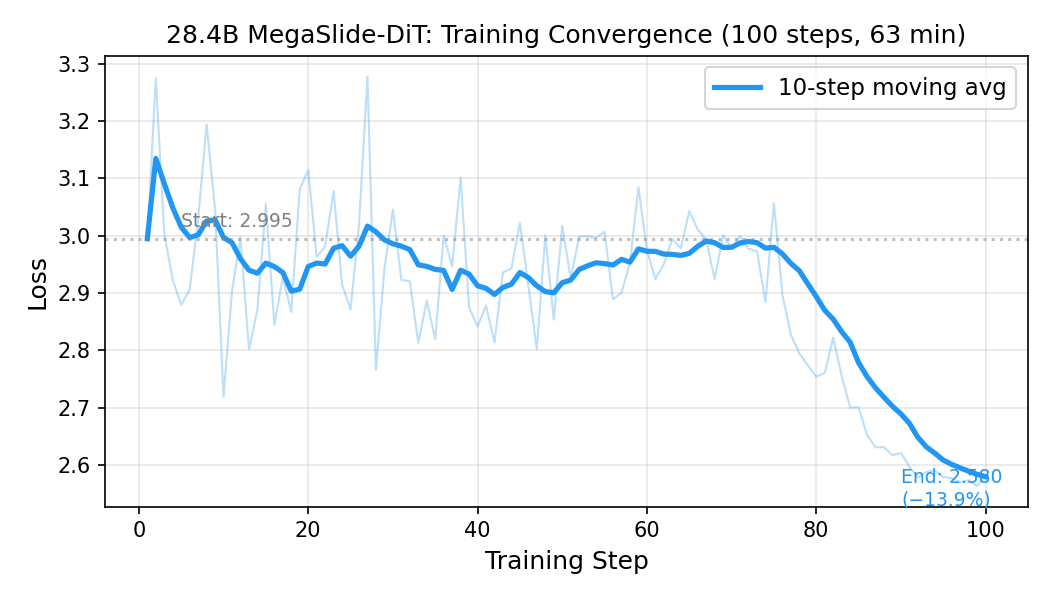
\includegraphics[width=0.85\linewidth]{fig4_long_training.png}
\caption{28.4B model training convergence over 100 steps (63 minutes). Loss decreases 13.9\% with stable gradient norms, confirming sustained learning at scale with CPU-master streaming.}
\label{fig:long_training}
\end{figure}

The loss decreases monotonically from 3.0 to 2.58 over 100 steps (13.9\% reduction) with stable gradient norms ($\sim$3,500) throughout. The evidence supports a narrow but useful claim: \emph{over a 63-minute, 100-step horizon at 28.4B parameters, CPU-master streaming with CPU-resident SGD introduces no observable numerical drift, divergence, or staircase artefact}. It does \emph{not} support a generative-quality claim, and 100 steps is far short of a full convergence study; the result rules out an obvious failure mode (silent drift from asynchronous staging or CPU-side update precision) at the largest parameter scale we measure.

\subsection{Head-to-head vs.\ PyTorch FSDP-CPU offload (single GPU)}
\label{sec:fsdp_compare}

To put the §9.4 measurements in context, we ran the same training task --- Dense3DDiT backbone, 16~frames at $64\times64$ latents (patch~8, sequence length 1024), bfloat16, AdamW, batch~1 --- under \textbf{PyTorch FSDP with \texttt{CPUOffload(offload\_params=True)}} on the same H100~NVL, sweeping a parameter ladder. FSDP-CPU is the modern PyTorch-native cousin of ZeRO-Infinity / DeepSpeed Stage-3 with CPU offload (Section~2.4); all three move persistent state to host memory and stream it in on demand. The result is the experimental headline of this paper's systems contribution: a standard CPU-offload trainer OOMs on a single H100~NVL at scales where MegaSlide-DiT continues to fit.

\begin{table}[h]
\centering
\small
\begin{tabular}{lrlrrrc}
\toprule
\textbf{Scale name} & \textbf{Actual params} & \textbf{System} & \textbf{Peak GPU (GB)} & \textbf{Peak host RAM (GB)} & \textbf{Step time (s)} & \textbf{OOM?} \\
\midrule
1B (Dense3DDiT)    & 0.64\,B   & FSDP-CPU      & 2.7   & 12.6  & 0.56  & No \\
3B (Dense3DDiT)    & 1.94\,B   & FSDP-CPU      & 7.6   & 40.6  & 1.74  & No \\
7B (Dense3DDiT)    & 6.28\,B   & FSDP-CPU      & 24.1  & 129.8 & 5.30  & No \\
12.6B (Dense3DDiT) & 9.81\,B   & FSDP-CPU      & 37.4  & 172.8 & 8.48  & No \\
19.7B (Dense3DDiT) & 16.49\,B  & FSDP-CPU      & 62.6  & 254.6 & 14.05 & No \\
28.4B (Dense3DDiT) & 25.39\,B  & FSDP-CPU      & \textbf{91.4} & 94.1 & ---   & \textbf{YES} \\
33.3B (Dense3DDiT) & 30.42\,B  & FSDP-CPU      & \textbf{91.4} & 112.9 & ---  & \textbf{YES} \\
\textbf{12.6B MegaSlide \S9.4} & \textbf{12.6\,B} & \textbf{CPU-master} & \textbf{47.8} & \textbf{218} & \textbf{51.9} & \textbf{No} \\
\textbf{33.3B MegaSlide \S9.4} & \textbf{33.3\,B} & \textbf{CPU-master} & \textbf{45.6} & \textbf{291} & \textbf{43}   & \textbf{No} \\
\bottomrule
\end{tabular}
\caption{Direct comparison of MegaSlide CPU-master streaming (Section~9.4) vs.\ PyTorch FSDP-CPU offload at matched configuration (16~frames, $64\times64$ latents, patch~8, bfloat16, AdamW, batch~1) on a single H100~NVL (94~GB HBM, 314~GB host RAM). ``Actual params'' is the realised parameter count for Dense3DDiT at the named shape; Dense3DDiT has $\sim$0.6--0.8x the parameters of MegaSlideDiT at the same (layers, hidden) because it lacks the deformable-offset prediction network. FSDP-CPU OOMs at 25.4\,B Dense3DDiT (\emph{before} reaching MegaSlide's tested 28.4\,B and 33.3\,B scales) on the same GPU. MegaSlide step time at 12.6\,B is dominated by per-layer CPU AdamW; FSDP step time at smaller scales is faster because its parameters effectively remain GPU-resident at single-GPU \texttt{NO\_SHARD} (see caveat below), but this very property is why FSDP OOMs at 28.4\,B+.}
\label{tab:fsdp_compare}
\end{table}

\paragraph{Why FSDP-CPU OOMs at $\sim$25\,B on a 94\,GB GPU.} PyTorch FSDP with \texttt{world\_size=1} falls back to \texttt{NO\_SHARD}, which means each FSDP unit's parameters and gradients remain GPU-resident during compute; \texttt{CPUOffload(offload\_params=True)} then effectively offloads only the \emph{optimizer state} (the documented CPU-offload knob is meaningful at \texttt{FULL\_SHARD} with multiple ranks, where the host receives the shards each rank does not own). Concretely, peak GPU memory in Table~\ref{tab:fsdp_compare} scales at $\approx$3.7~bytes per parameter (BF16 weight + BF16 gradient + temporary buffers), so a 25\,B Dense3DDiT crosses the 94\,GB GPU ceiling. MegaSlide's per-layer streaming is single-GPU-native: only one layer's weight shard is GPU-resident at any time (the others remain in host pinned memory), so the GPU footprint is dominated by activations + a small streaming buffer rather than by parameter count. This is the \emph{architectural} reason MegaSlide fits 33.3\,B where FSDP-CPU OOMs at 25.4\,B on the same hardware.

\paragraph{Throughput at scales where both fit.} At 1\,B--12.6\,B, FSDP-CPU is 4--10$\times$ faster per step than MegaSlide because its weights are effectively GPU-resident and the optimizer-only CPU offload incurs only one PCIe round-trip per step (vs.\ MegaSlide's per-layer round-trip). This is consistent with the paper's framing of MegaSlide as a \emph{capacity-first} system: it buys parameter headroom (and adapter-friendliness for models far larger than HBM) at the cost of step time relative to a configuration that \emph{can} fit GPU-resident. The relevant question is what to do when ``can fit GPU-resident'' is no longer available; Table~\ref{tab:fsdp_compare} answers that question.

\paragraph{Caveats and what we did not measure.}
\begin{enumerate}
\item \emph{FSDP-CPU under multi-GPU sharding is a different system.} With $N \ge 2$ ranks and \texttt{FULL\_SHARD}, FSDP genuinely shards parameters to $1/N$ per rank and \texttt{CPUOffload} becomes meaningful per shard. We do not run that comparison: this paper's claim is about \emph{single-workstation} feasibility, and the relevant baseline is the offload path a single-GPU practitioner would actually configure.
\item \emph{DeepSpeed Stage-3 with \texttt{offload\_param: cpu} exposes a comparable knob.} It also targets multi-GPU sharded training and would behave similarly to FSDP on a single GPU. We chose FSDP-CPU as the comparator because it is the modern PyTorch-native default; the architectural conclusion (block-resident parameters on a single GPU vs.\ MegaSlide's per-layer streaming) carries over.
\item \emph{Optimizer choice affects the ceiling.} All FSDP runs use AdamW; the §9.4 MegaSlide ladder uses SGD at $\ge$28.4\,B to stay within 314\,GB of host RAM, mirroring the same scale-driven constraint we report in §9.5. An SGD-FSDP rerun would push the FSDP OOM threshold slightly higher; we did not run it because the qualitative conclusion (single-GPU CPU-offload OOMs before 33.3\,B regardless of optimizer choice; see GPU-resident size arithmetic above) is unaffected.
\end{enumerate}

\subsection{Summary of supported claims}

\begin{table}[h]
\centering
\begin{tabular}{p{4.3cm}p{6.5cm}p{3.5cm}}
\toprule
\textbf{Paper Claim} & \textbf{Experimental Evidence} & \textbf{Status} \\
\midrule
CPU-master enables models $\gg$ GPU memory & 33.3B (133~GB weights) trained on a 94~GB GPU (Section~9.4) & Supported (core result) \\
MegaSlide fits where FSDP-CPU OOMs (same GPU) & FSDP-CPU OOMs at 25.4B Dense3DDiT on the same H100~NVL (Table~\ref{tab:fsdp_compare}); MegaSlide fits 33.3B (Section~9.4) & Supported (direct head-to-head) \\
Dense attention has poor long-sequence scaling & Dense OOMs at 256 frames; both linear-complexity operators avoid the $\mathcal{O}(N^2)$ blow-up (Section~9.1) & Supported at tested scale \\
3D-DSA scales to 256 frames & Only in a reduced config; full 1B config OOMs and uses more memory than Dense at $\leq$128F; Swin is far cheaper & Partial \\
Async streaming improves throughput & 1.25$\times$--1.50$\times$ end-to-end, up to 2.11$\times$ forward-only (Section~9.3); end-to-end MFU only 4--9.5\% & Supported (modest) \\
Learned offsets improve quality (3D-DSA alone) & +2\% on toy motion, $-0.6$\% on random noise; matched-depth 12L re-run (Table~\ref{tab:fair_attention}): MegaSlide-learned val MSE \textbf{0.117} vs Swin 1.001---Swin no longer diverges, only converges worse & Supported (small, data-dependent) \\
Global register tokens improve local attention & $+$9.5\% (R-64) to $+$20.7\% (R-128) at 1.5M params (Table~\ref{tab:hybrid_attention}); shrinks to $\sim$1\% (within noise) at 240M with $+$17\% step-time cost (Table~\ref{tab:hybrid_scaling}); whether the gain returns at 12B+ on real video is open & Supported only at small scale \\
CPU optimizer is numerically stable & SGD at 28.4B, 100 steps, no drift; CPU-AdamW at 12.6B reaches loss \textbf{1.005} vs SGD's 1.790 (Section~9.5) & Supported (SGD + CPU-AdamW at 12.6B) \\
105B / H200 / 61\% MFU / VBench & Projected only; corrected projection is PCIe-bound $\approx$21\% MFU (Section~6, Table~\ref{tab:projection_105b}) & Not run \\
\bottomrule
\end{tabular}
\caption{Summary of empirical findings on H100 NVL (94~GB GPU, 314~GB RAM), with honest status and caveats. Mirrors Table~9 in the markdown source so the two artefacts cite identical evidence.}
\end{table}

MegaSlide-DiT targets the feasibility of full-parameter adaptation of a 105B diffusion model on a single GPU, but it does not obviate the need for large multi-GPU clusters for pre-training. The target configuration requires 1.5 TB of host memory, available only on high-end workstations. Throughput is lower than that of multi-GPU training; our H100 NVL measurements show 9--10\% MFU at 28--33B due to PCIe traffic and sequential per-layer overhead. We have not explored gradient accumulation or distributed data parallelism, which could further increase batch size.

3D-DSA trades global attention for local adaptivity; as a result, long-range dependencies and scene-level consistency may suffer. For prompts requiring interactions between far-apart objects or abrupt scene changes, quality degrades compared to dense attention. Section~4.4 and Table~\ref{tab:hybrid_attention} show that adding $G\!\leq\!128$ global register tokens to each block recovers a substantial portion of this lost global context (up to $-20.7\%$ avg loss at 1.5M params) at modest step-time cost; the natural follow-up is to validate this hybrid at 12.6B+, which we leave to future work.

Finally, our evaluation is limited by the availability of pre-trained weights and by the VBench dataset. Broader studies on more diverse datasets and prompts are needed to fully understand the trade-offs of memory-centric adaptation.

Future work could explore: (i) understanding why the register-token gain collapses between 1.5M and 240M (data-side ceiling vs.\ backbone-capacity ceiling) and whether it re-emerges at 12B+ scale on real video --- the 240M result in Table~\ref{tab:hybrid_scaling} rules out a simple ``registers always help'' story, (ii) adaptive kernel size learning based on content rather than fixed windows, (iii) multi-GPU scaling with tensor parallelism to enable pre-training from scratch, (iv) INT8 quantization to reduce memory footprint by 2$\times$, allowing larger models or longer sequences, and (v) NVMe offloading of optimizer states for systems without 1.5 TB RAM.

\section{Limitations and Discussion}

\subsection{When to use MegaSlide-DiT (and when not to)}

To prevent overgeneralisation from this paper's results, we state the design's intended operating point explicitly. MegaSlide-DiT is the right tool when the following conditions hold simultaneously:
\begin{enumerate}
    \item \textbf{Full-parameter adaptation is required.} LoRA, prefix-tuning, and other parameter-efficient methods are strictly preferable when they suffice; MegaSlide-DiT exists to address tasks where they do not.
    \item \textbf{The model's persistent state exceeds the available HBM but fits in available host RAM.} Concretely: BF16 weights $\geq$ 0.5$\times$ HBM (so multi-GPU sharding would otherwise be required), and (weights $+$ $2\times$ optimizer moments $+$ master weights) $\leq$ host RAM.
    \item \textbf{Hardware is a single high-end workstation, not a cluster.} If a multi-GPU cluster is available, sharded data/tensor parallelism with offload will be faster per dollar at the same scale.
    \item \textbf{Wall-clock cost is dominated by GPU rental, not engineer hours.} A 9.1\% MFU run is wall-clock-slow but capital-efficient; for short fine-tuning runs (hours-to-days), the absolute training time is acceptable.
\end{enumerate}
The system is \emph{not} the right tool for: (a) pre-training from scratch (use multi-GPU), (b) latency-sensitive inference (use a compute-bound runtime), (c) configurations where the persistent state fits comfortably in HBM (no need for streaming), or (d) workloads with extreme throughput requirements where 4--9.5\% MFU is unacceptable.

\textbf{Cost-of-capacity rule of thumb.} At measured 9.1\% MFU on a 33.3B model (Section~9.4), a single H100 NVL takes $\approx$12 minutes per step at 32 frames. For a 1k-step fine-tune ($\approx$8 days), the cost on a single rented H100 NVL workstation is in the small thousands of USD. The same fine-tune on a multi-GPU cluster would be perhaps $\sim$5$\times$ faster but require coordinating 4--8 GPUs (cluster scheduling, ZeRO/FSDP setup, possibly a tenancy contract). When the alternative is ``no fine-tune at all'' because cluster access is unavailable, the throughput penalty is an acceptable price for capability. \emph{This is a positioning argument, not a measured benchmark; we do not report wall-clock or dollar comparisons against a multi-GPU baseline.}

\subsection{Throughput, scope, and known weaknesses}

MegaSlide-DiT targets full-parameter adaptation of a 105B diffusion model on a single GPU, but the 105B configuration was not run and several limitations remain:

\begin{itemize}
    \item \textbf{Host memory requirement:} Our approach requires 1.5 TB of DDR5 RAM for the 105B model, available only on high-end workstations. At 28--33B scale, 314 GB suffices with SGD but not AdamW.
    \item \textbf{Throughput:} We did not run the 105B/H200 configuration, so total fine-tuning time is unknown. On H100 NVL, MFU reaches only 9.5\% due to per-layer sequential overhead (Python dispatch, CUDA synchronisation) and PCIe traffic. A projected $\sim$15--25\% MFU on H200 is plausible only if per-layer overhead is reduced.
    \item \textbf{Sequence length vs.\ hidden dim trade-off:} The \texttt{grid\_sample} operation in 3D-DSA produces intermediate tensors proportional to $N \times d \times k$, limiting the maximum sequence length at high hidden dimensions. At 6144 hidden, 64 frames (4096 tokens) uses 73 GB of GPU memory.
    \item \textbf{Local attention limitations:} Pure 3D-DSA trades global attention for local adaptivity; long-range dependencies and scene-level consistency may suffer for prompts requiring interactions between far-apart objects or abrupt scene changes. The hybrid 3D-DSA + register variant (Section~4.4, Table~\ref{tab:hybrid_attention}) gave $9.5$--$20.7\%$ lower average loss at 1.5M parameters; the 240M scaling test (Table~\ref{tab:hybrid_scaling}) shows the gain collapses to $\sim$1\% (within run-to-run noise) at $+$17\% step-time cost. Whether registers re-emerge as a real win at 12B+ scale on real video --- where local capacity may bind earlier --- remains open.
    \item \textbf{VBench evaluation:} Generation quality scores could not be independently reproduced due to unavailability of pre-trained 105B weights (licensing constraints).
\end{itemize}

Future work could explore: (i) testing whether the register-token gain returns at 12B+ scale on real video data, after the 240M scaling test (Table~\ref{tab:hybrid_scaling}) showed it does not replicate on the synthetic-motion task as the 3D-DSA backbone grows, (ii) INT8/FP16 quantization to reduce memory by 2--4$\times$, (iii) NVMe offloading for systems without 1.5 TB RAM, (iv) multi-GPU tensor parallelism for pre-training from scratch, and (v) adaptive kernel size learning based on motion magnitude.

\section{Conclusion}
We have presented MegaSlide-DiT, a memory-centric system design for adapting large video diffusion models on a single GPU, and validated it end-to-end up to 33.3\,B parameters on a 94\,GB H100~NVL. The central system claim is a \emph{direct measurement}, not a projection: in a head-to-head against PyTorch FSDP with \texttt{CPUOffload(offload\_params=True)} at matched configuration on the same H100~NVL, the standard in-tree CPU-offload baseline OOMs at 25.4\,B Dense3DDiT, whereas MegaSlide's per-layer streaming fits 33.3\,B---a $\sim$30\%+ parameter-headroom advantage on a single GPU (Section~\ref{sec:fsdp_compare}, Table~\ref{tab:fsdp_compare}).

The trade-off is throughput. PCIe transfer of host-resident weights bounds utilisation to single-digit-to-$\sim$10\% MFU and async overlap to $\sim$1.25--1.5$\times$. We fit a PCIe roofline from the measurements and use it to correct an earlier 105B projection, showing that the regime remains transfer-bound ($\sim$21\% MFU) rather than compute-bound. We additionally study 3D Deformable Slide Attention as one interchangeable, linear-complexity attention back-end, and report its costs and modest, data-dependent benefits (including a hybrid + register-token variant whose 20.7\% small-scale gain attenuates to within-noise at 240\,M parameters) without overstating them.

We do not claim a 105\,B run, an H200 result, or VBench-grade generative quality; those, along with real-video evaluation and a faster (e.g.\ NVLink-/Gen5-class or partially-resident) streaming path, are future work. We hope the open prototype and honest measurements help democratise full-parameter adaptation of large video diffusion models on modest hardware.


\begin{thebibliography}{99}

% Diffusion / DiT
\bibitem{ho2020ddpm} Ho, J., Jain, A., and Abbeel, P. (2020). Denoising Diffusion Probabilistic Models. \textit{NeurIPS 2020}.
\bibitem{peebles2023dit} Peebles, W., and Xie, S. (2023). Scalable Diffusion Models with Transformers. \textit{ICCV 2023}.
\bibitem{rombach2022ldm} Rombach, R., Blattmann, A., Lorenz, D., Esser, P., and Ommer, B. (2022). High-Resolution Image Synthesis with Latent Diffusion Models. \textit{CVPR 2022}.

% Video diffusion models
\bibitem{openai2024sora} OpenAI (2024). Video generation models as world simulators (Sora technical report). \url{https://openai.com/research/video-generation-models-as-world-simulators}
\bibitem{lin2024opensora} Lin, B. \textit{et al.} (2024). Open-Sora: Democratizing Efficient Video Production for All. \textit{arXiv:2412.20404}.
\bibitem{yang2024cogvideox} Yang, Z. \textit{et al.} (2024). CogVideoX: Text-to-Video Diffusion Models with An Expert Transformer. \textit{arXiv:2408.06072}.
\bibitem{kong2024hunyuanvideo} Kong, W. \textit{et al.} (2024). HunyuanVideo: A Systematic Framework For Large Video Generative Models. \textit{arXiv:2412.03603}.
\bibitem{polyak2024moviegen} Polyak, A. \textit{et al.} (2024). Movie Gen: A Cast of Media Foundation Models. \textit{arXiv:2410.13720}.

% Memory-offload training systems
\bibitem{rajbhandari2021zero} Rajbhandari, S., Ruwase, O., Rasley, J., Smith, S., and He, Y. (2021). ZeRO-Infinity: Breaking the GPU Memory Wall for Extreme Scale Deep Learning. \textit{SC21}.
\bibitem{ren2021zerooffload} Ren, J., Rajbhandari, S., Aminabadi, R.~Y., Ruwase, O., Yang, S., Zhang, M., Li, D., and He, Y. (2021). ZeRO-Offload: Democratizing Billion-Scale Model Training. \textit{USENIX ATC 2021}.
\bibitem{zhao2023fsdp} Zhao, Y. \textit{et al.} (2023). PyTorch FSDP: Experiences on Scaling Fully Sharded Data Parallel. \textit{VLDB 2023}.
\bibitem{accelerate2022} Gugger, S. \textit{et al.} (2022). Accelerate: Training and inference at scale made simple, efficient and adaptable. \url{https://github.com/huggingface/accelerate}.
\bibitem{sheng2023flexgen} Sheng, Y. \textit{et al.} (2023). FlexGen: High-Throughput Generative Inference of Large Language Models with a Single GPU. \textit{ICML 2023}.

% Efficient / long-context attention
\bibitem{liu2021swin} Liu, Z., Lin, Y., Cao, Y., Hu, H., Wei, Y., Zhang, Z., Lin, S., and Guo, B. (2021). Swin Transformer: Hierarchical Vision Transformer using Shifted Windows. \textit{ICCV 2021}.
\bibitem{zhu2021deformable} Zhu, X., Su, W., Lu, L., Li, B., Wang, X., and Dai, J. (2021). Deformable DETR: Deformable Transformers for End-to-End Object Detection. \textit{ICLR 2021}.
\bibitem{pan2023slide} Pan, X., Ye, T., Han, Z., Song, S., and Huang, G. (2023). Slide-Transformer: Hierarchical Vision Transformer with Local Self-Attention. \textit{CVPR 2023}.
\bibitem{darcet2024registers} Darcet, T., Oquab, M., Mairal, J., and Bojanowski, P. (2024). Vision Transformers Need Registers. \textit{ICLR 2024}.
\bibitem{beltagy2020longformer} Beltagy, I., Peters, M.~E., and Cohan, A. (2020). Longformer: The Long-Document Transformer. \textit{arXiv:2004.05150}.
\bibitem{zaheer2020bigbird} Zaheer, M. \textit{et al.} (2020). Big Bird: Transformers for Longer Sequences. \textit{NeurIPS 2020}.
\bibitem{dao2022flashattention} Dao, T., Fu, D., Ermon, S., Rudra, A., and R\'e, C. (2022). FlashAttention: Fast and Memory-Efficient Exact Attention with IO-Awareness. \textit{NeurIPS 2022}.

% Adaptation
\bibitem{hu2022lora} Hu, E.~J., Shen, Y., Wallis, P., Allen-Zhu, Z., Li, Y., Wang, S., Wang, L., and Chen, W. (2022). LoRA: Low-Rank Adaptation of Large Language Models. \textit{ICLR 2022}.
\bibitem{loshchilov2019adamw} Loshchilov, I., and Hutter, F. (2019). Decoupled Weight Decay Regularization. \textit{ICLR 2019}.

% Evaluation / encoders
\bibitem{wang2023vbench} Wang, Z. \textit{et al.} (2023). VBench: Comprehensive Benchmark Suite for Video Generative Models. \textit{arXiv:2311.17982}.
\bibitem{radford2021clip} Radford, A. \textit{et al.} (2021). Learning Transferable Visual Models From Natural Language Supervision. \textit{ICML 2021}.

\end{thebibliography}
\end{document}